\section{Setting}
\ourgame{} is set primarily in the modern age, in a world very much like the player's own. The main environment is Omar Clean's mansion. From the outside, the mansion is a decently large Palladian-inspired building, similar to Figure~\ref{fig:mansion_photo}. On the inside, the rooms are modestly sized, conservatively designed, and unassuming. However, as one explores the rooms of the mansion, it becomes clear that it is larger on the inside than the outside. Much, much larger. Impossibly large. And doors start to lead to impossible places, like giant forests, or dockside crime lairs.

\begin{figure}[htb]
\centering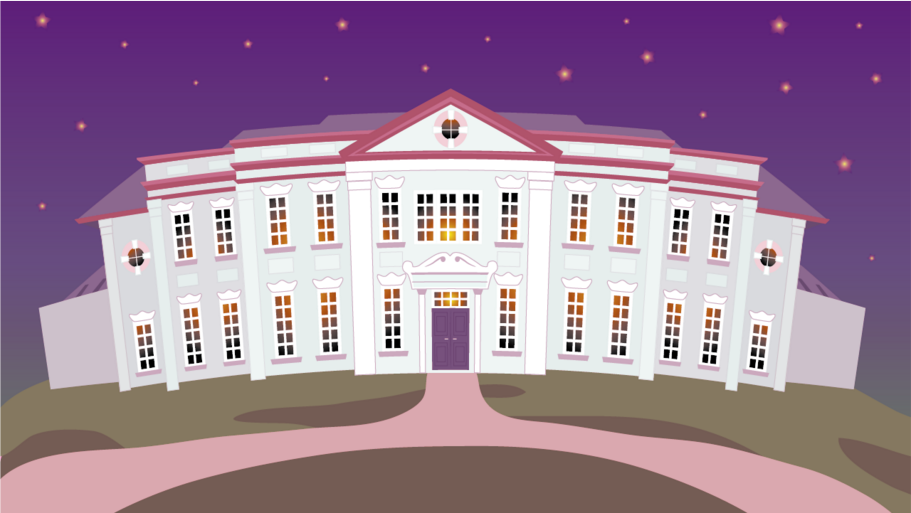
\includegraphics[width=.4\linewidth]{images/mansion2}
\caption{Concept artwork of Omar's mansion, inspired by neo-Palladian English architecture.}
\label{fig:mansion_photo}
\end{figure}

The game environment is rendered in 3D using a stylized cartoon aesthetic. It is populated by many unique characters. Most appear to be human but it is clear that the inhabitants of this world are more than they seem. They can have brightly-coloured skin, outrageous body types, and even animal parts. The characters are rendered in the game environment as 2D billboards to create an off-kilter visual style, similar to those in Figure~\ref{fig:render_style}.

\begin{figure}[htb]
  \centering%
  \begin{subfigure}{.33\textwidth}
    \centering
    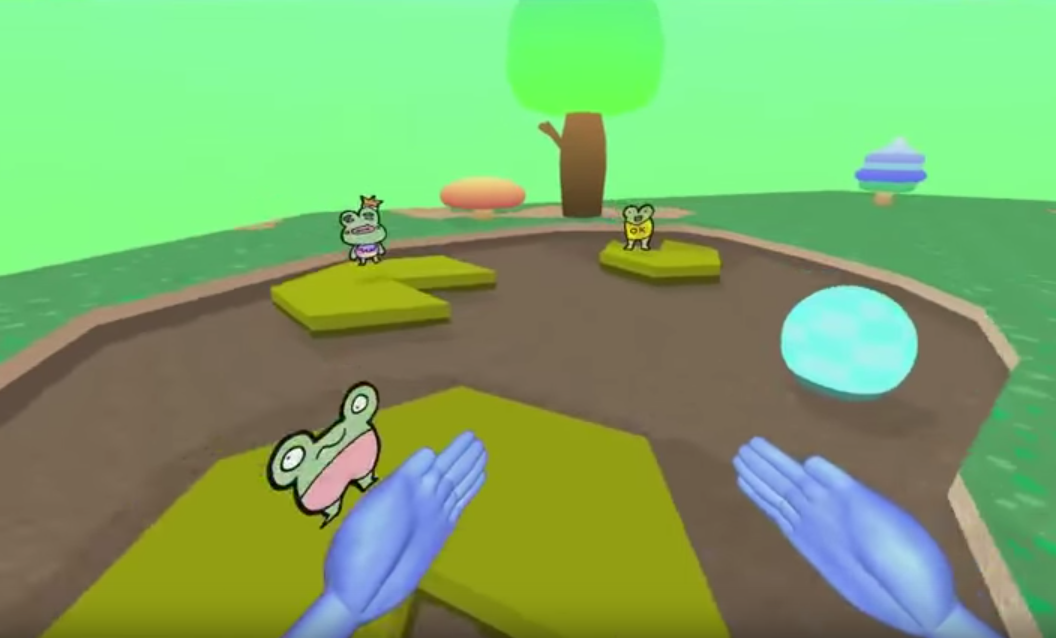
\includegraphics[width=.9\linewidth]{images/burrito}
  \end{subfigure}%
  \begin{subfigure}{.33\textwidth}
    \centering
    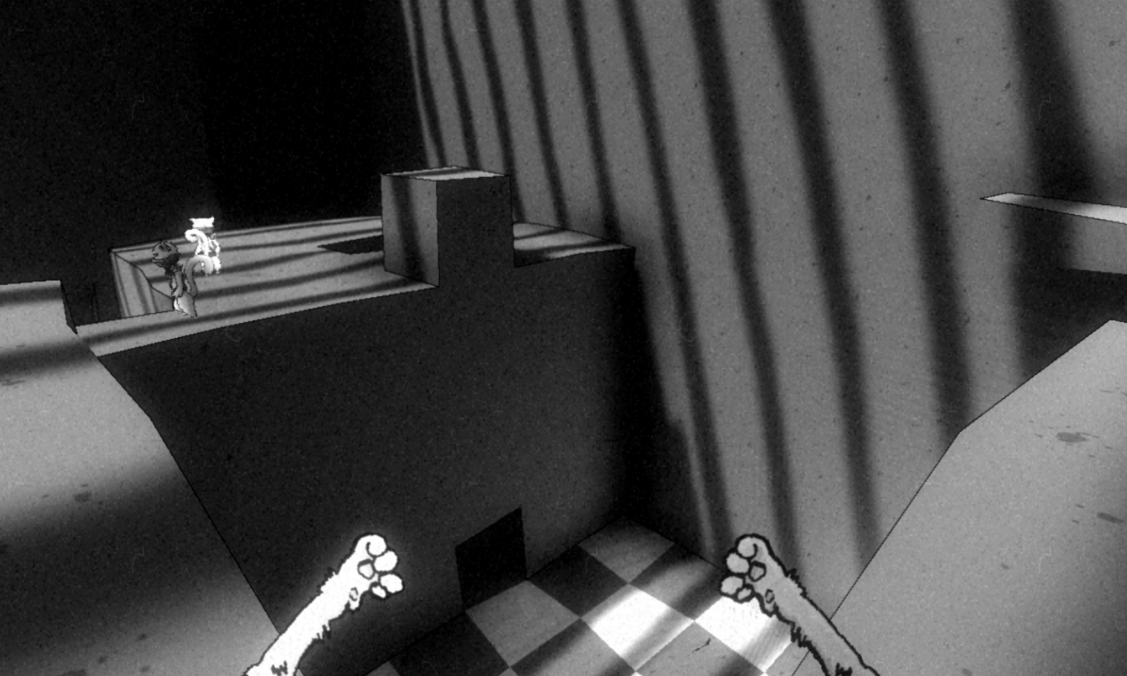
\includegraphics[width=.9\linewidth]{images/sketchtales}
  \end{subfigure}%
  \caption{The upcoming games \textit{Burrito Galaxy 65} and \textit{Sketch Tales} both render 2D characters in stylized and cartoon 3D worlds.}
  \label{fig:render_style}
\end{figure}

Throughout the game, the player can travel to alternate dimensions. Every playthrough occurs within Omar Clean's mansion, but the mansion changes in subtle ways. The style and interior design remain the same, but the floor layout, furniture, items, and character designs all change and shift between dimensions. The mansion is always owned by Omar Clean, but each dimension has its own unique version of Omar -- sometimes an adventurer, sometimes a scientist, sometimes a robot. 

The protagonist of \ourgame{} is a blank slate. The player controls this character, and can project their own impressions and assumptions with them into the world, which shapes the way they interpret their surroundings, and their purpose within \ourgame{}.